\chapter{Hardware}

%TODO: Mention initial parts list was inspired by http://www.instructables.com/id/Autonomous-Lynxmotion-Rover/
\section{Specific Hardware Used}

\begin{wrapfigure}{r}{0.25\textwidth} %this figure will be at the right
	\caption{Lynxmotion 4WD Rover \cite{fig_lynxmotion_rover}}
	\centering
	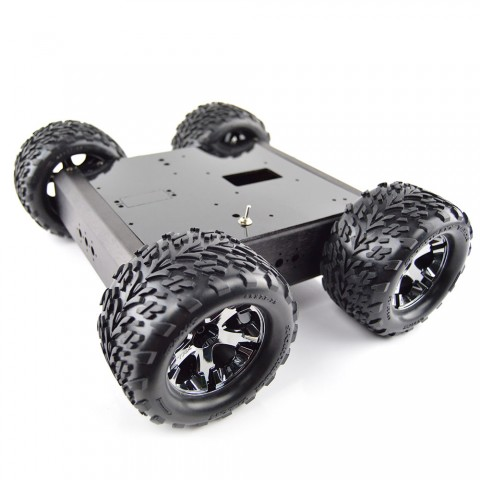
\includegraphics[width=0.25\textwidth]{lynxmotion-aluminum-a4wd1-rover-kit-w-encoders-7}
\end{wrapfigure}

The mobile base used is the Lynxmotion A4WD1 Rover, shown on the right. This kit comes with four 200 rpm dc gear motors, and four optical quadrature motor encoders.

\begin{wrapfigure}{l}{0.25\textwidth}
	\caption{Sabertooth 2x12 \cite{fig_sabertooth}}
	\centering
	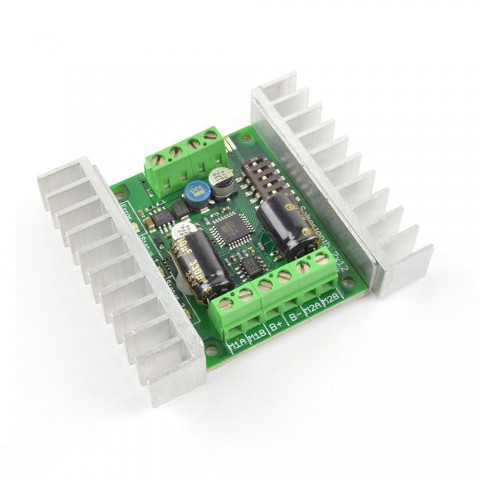
\includegraphics[width=0.25\textwidth]{sabertooth-dual-regenerative-motor-driver_3}
\end{wrapfigure}

The motors are controlled by a Sabertooth dual-channel 12A 6V-24V regenerative motor driver, shown on the left. This motor driver is powered by two LG 18650 HE2 rechargable lithium ion cells, which sit in an 18650 battery case which has been soldered to act as a battery pack with two 18650 cells in series. The battery cells are individually charged before use with a NiteCore-i2-V2014 li-ion charger.

\begin{wrapfigure}{r}{0.25\textwidth} %this figure will be at the right
	\caption{PING))) Ultrasonic Sensor \cite{fig_ping}}
	\centering
	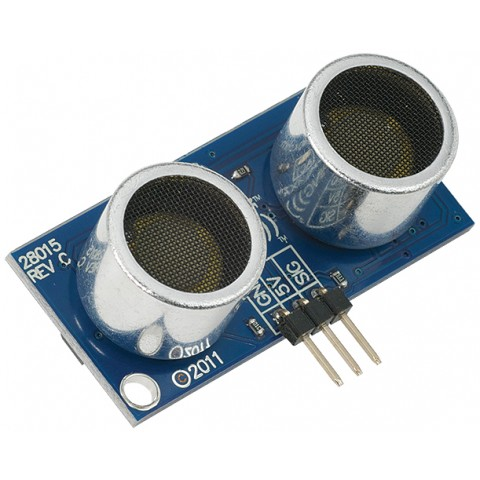
\includegraphics[width=0.25\textwidth]{parallax-ping-ultrasonic-sensor_1}
\end{wrapfigure}

On top of the rover is the PING))) ultrasonic distance sensor, which is attached to a standard Parallax servo which pans back and forth 180 degrees.

\begin{wrapfigure}{l}{0.25\textwidth}
	\caption{Arduino Uno R3 \cite{fig_arduino_uno}}
	\centering
	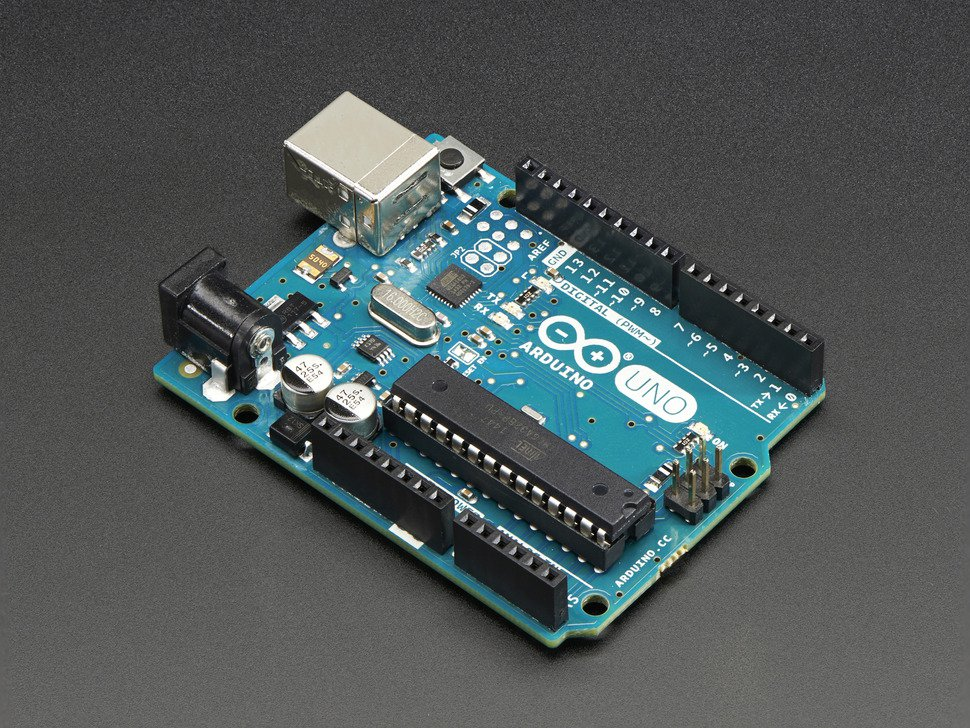
\includegraphics[width=0.25\textwidth]{arduinoUno}
\end{wrapfigure}

At the center of the rover is an Arduino Uno R3. This microcontroller handles several important tasks. It tells the motor driver what speed to set its two output channels to, and directly controls the panning motion of the standard Parallax servo. It also acts as a go-between for the digital output of the sensors on the rover and a laptop. It's connected to this laptop via a USB cable, which powers the board and allows communication over a serial port. Motor encoder values and ultrasonic range data are transmitted to the laptop, and motor power commands are received.

The specific laptop used in this project is the Dell Inspiron 3531, which has a quad core 2.16 GHz processor, and 4 GB of RAM. While these are relatively limited computational resources, the laptop was a personal work machine and already available to use for no additional cost. The machine is used as the main processing unit for the navigation logic. 

The last component is a Nexus 4 smartphone placed on the top panel of the rover, which is also connected to the laptop by USB. Inside this phone is an MPU-6050 chip which contains a gyroscope and accelerometer. Elsewhere on the phone's logic board are a magnetometer, otherwise known as a digital compass, and a GPS receiver. This smartphone was also already available, and acts as a cheap Inertial Measurement Unit (IMU) and GPS receiver for the robot.

\section{Construction}

\begin{figure}[h]
	\caption{Connections Made}
	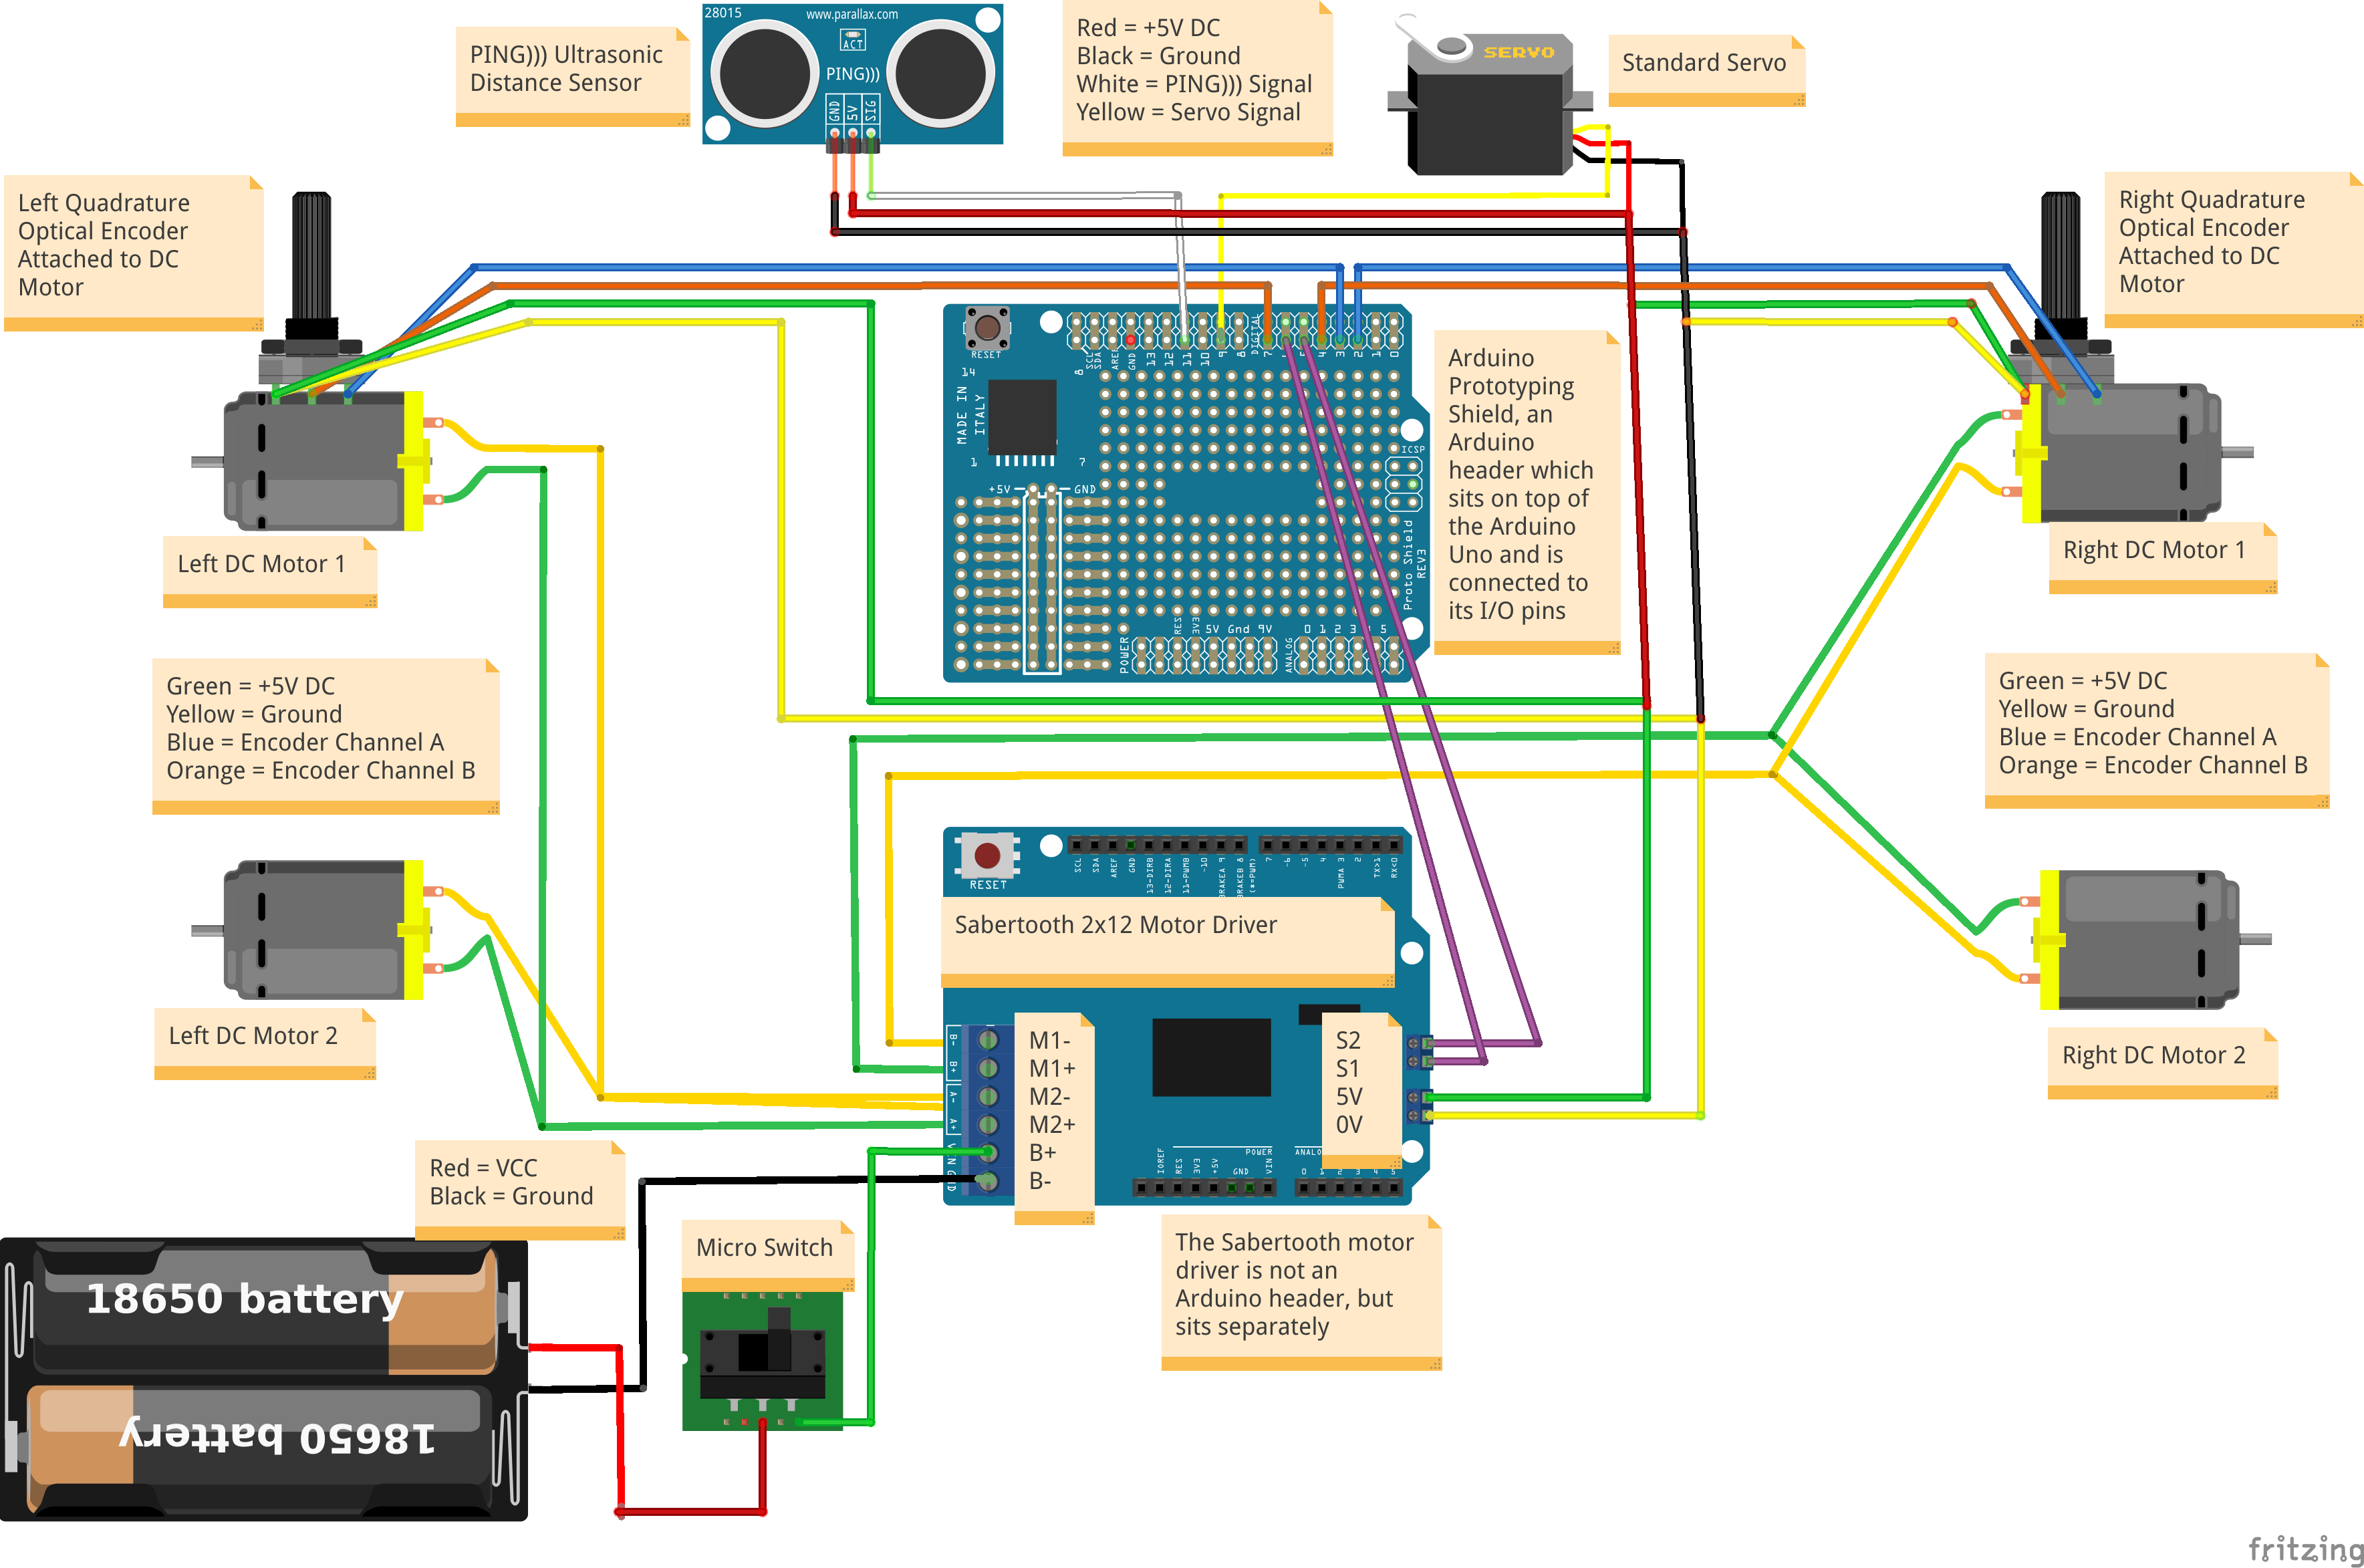
\includegraphics[width=\textwidth,height=\textheight,keepaspectratio]{RoverDesign}
	\centering
	\text{This image was created with Fritzing.}
\end{figure}

\subsection{Arduino Pin Connections}
Most digital pin numbers used are arbitrary, and connections may be permuted without any change. The sole exception  for Special care is taken in the 

\section{Arduino Sketch}
A sketch is Arduino-speak for a program uploaded to the board which will run on a loop as long as the board is powered.
